% 06-language-model-exploration-appendix.tex

% Section Title
\section{LANGUAGE MODEL EXPLORATION}

    % Main Content
    
    \subsection{Training Configuration}

        The model was implemented using BERT (bert-base-uncased) with the following key configurations:
        \begin{itemize}
            \item Maximum sequence length: 128 tokens
            \item Learning rate: 4e-5 with AdamW optimizer ($\beta_1=0.9$, $\beta_2=0.98$, $\epsilon=1e-6$)
            \item Training epochs: 4
            \item Gradient accumulation steps: 4
            \item Mixed precision training enabled
            \item Linear learning rate scheduler without warmup
            \item Loss function: Binary Cross-Entropy with Logits
        \end{itemize}
        
    \subsection{Model Performance Metrics}

        \subsubsection{3D ROC Analysis}

            The 3D ROC curve (Figure \ref{fig:3d_roc}) illustrates:

            \begin{itemize}
                \item Superior performance for Execution class (green line)
                \item Strong performance for Discovery class (orange line)
                \item Slightly lower but still good performance for Defense Evasion (blue line)
            \end{itemize}

        \subsubsection{Class-wise F1 Scores}
        
            The model demonstrates varying performance across classes (Figure \ref{fig:f1_scores}):

            \begin{itemize}
                \item Excellent performance (F1 $\geq$ 0.98) for Defense Evasion, Discovery, Execution, Other, and Persistence classes
                \item Perfect scores (F1 = 1.00) for Discovery and Persistence
                \item Significantly lower performance for Harmless class (F1 = 0.22)
                \item Impact class shows minimal detection capability (F1 = 0.00)
            \end{itemize}

        \subsubsection{Detailed Performance Metrics}

            The performance metrics (Figure \ref{fig:performance_metrics}) reveal:

            \begin{itemize}
                \item Most classes achieve balanced precision and recall scores
                \item The Harmless class shows a significant disparity between precision and recall
                \item The Impact class shows minimal performance across all metrics
            \end{itemize}

        \subsubsection{Precision-Recall Analysis}

            The Precision-Recall curves (Figure \ref{fig:pr_curves}) demonstrate:

            \begin{itemize}
                \item Most classes maintain high precision (>0.95) across different recall thresholds
                \item The "Other" category shows a sharp decline in precision at approximately 0.2 recall
                \item Impact and Harmless classes demonstrate poor precision-recall trade-offs
                \item Defense Evasion, Discovery, Execution, and Persistence maintain near-perfect precision until very high recall values
            \end{itemize}

        \subsubsection{Prediction Probability Distribution}

            The prediction probability histograms (Figure \ref{fig:pred_prob}) reveal:

            \begin{itemize}
                \item Most classes exhibit a strong binary separation in prediction probabilities
                \item Defense Evasion, Discovery, and Execution show high-confidence predictions clustered near 0 and 1
                \item The Persistence class shows a similar pattern but with a smaller proportion of low-probability predictions
                \item Harmless and Impact classes show predominantly low-probability predictions, indicating potential class imbalance issues
            \end{itemize}
            
        \begin{figure}[h]
            \centering
            \begin{minipage}[c]{0.47\textwidth}
                \centering
                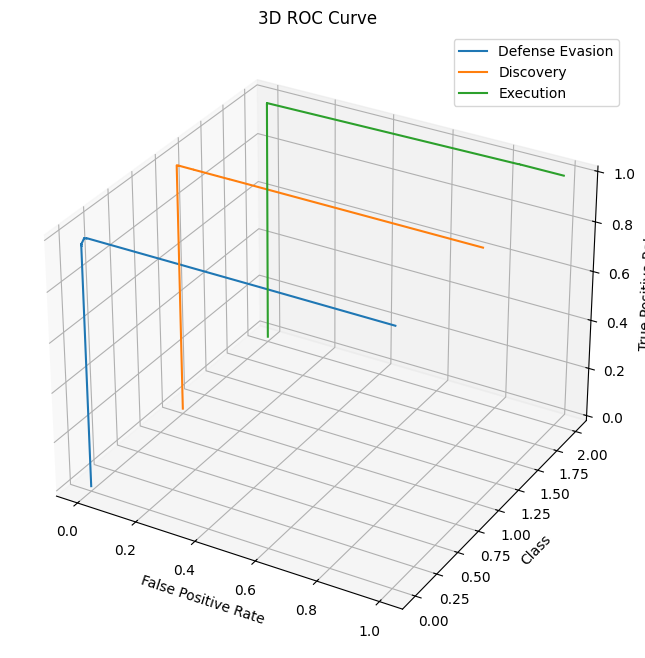
\includegraphics[width=0.6\textwidth]{../figures/plots/section4/3d_roc_curve.png}
                \caption{3D ROC curves showing the performance trade-off between true positive rate and false positive rate across different classification thresholds for Defense Evasion, Discovery, and Execution classes.}
                \label{fig:3d_roc}
            \end{minipage}
            \hfill
            \begin{minipage}[c]{0.47\textwidth}
                \centering
                \vspace{0.1cm}
                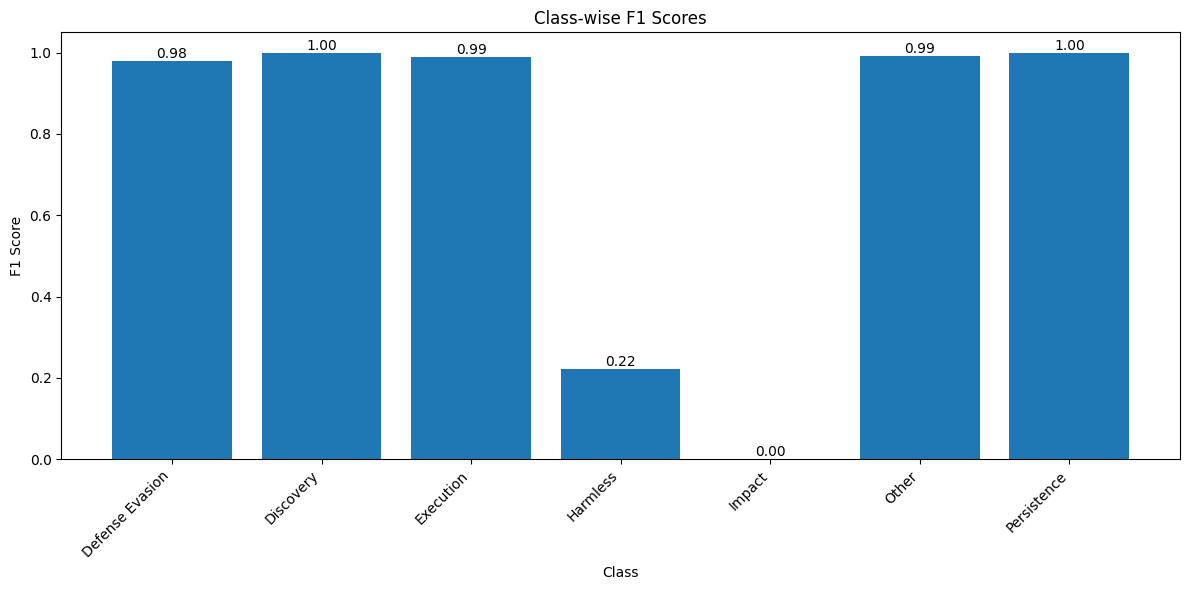
\includegraphics[width=\textwidth]{../figures/plots/section4/f1_scores.png}
                \caption{F1 scores across different classes showing the model's classification performance for each category.}
                \label{fig:f1_scores}
            \end{minipage}
        \end{figure}
        
        \begin{figure}[h]
            \centering
            \begin{minipage}[c]{0.47\textwidth}
                \centering
                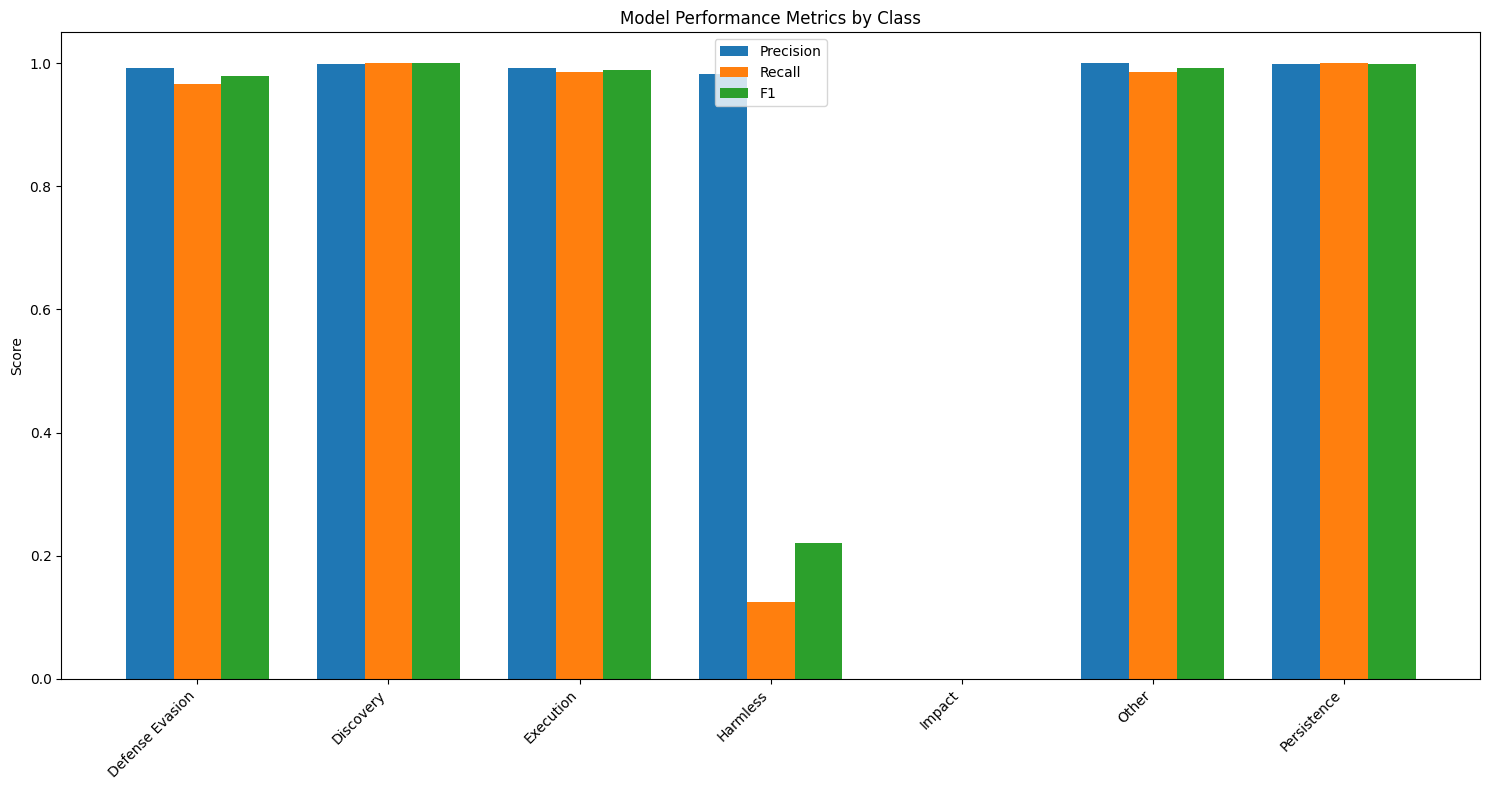
\includegraphics[width=\textwidth]{../figures/plots/section4/performance_metrics.png}
                \caption{Detailed breakdown of Precision, Recall, and F1 scores for each class.}
                \label{fig:performance_metrics}
            \end{minipage}
            \hfill
            \begin{minipage}[c]{0.47\textwidth}
                \centering
                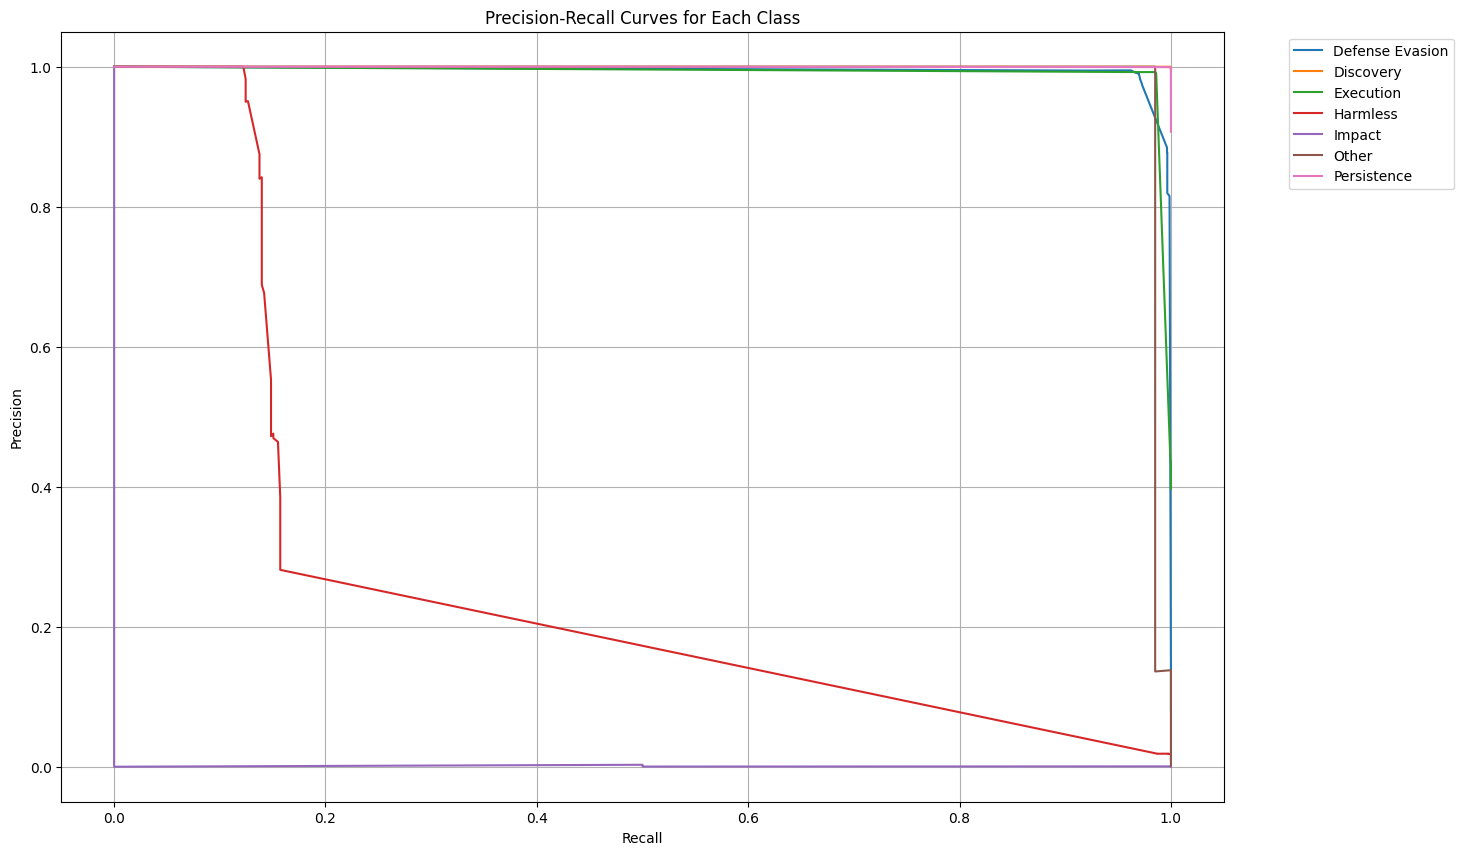
\includegraphics[width=\textwidth]{../figures/plots/section4/precision_recall_curves.png}
                \caption{Precision-Recall curves for each class showing the trade-off between precision and recall at different classification thresholds.}
                \label{fig:pr_curves}
            \end{minipage}
        \end{figure}
        
        \begin{figure}[h]
            \centering
            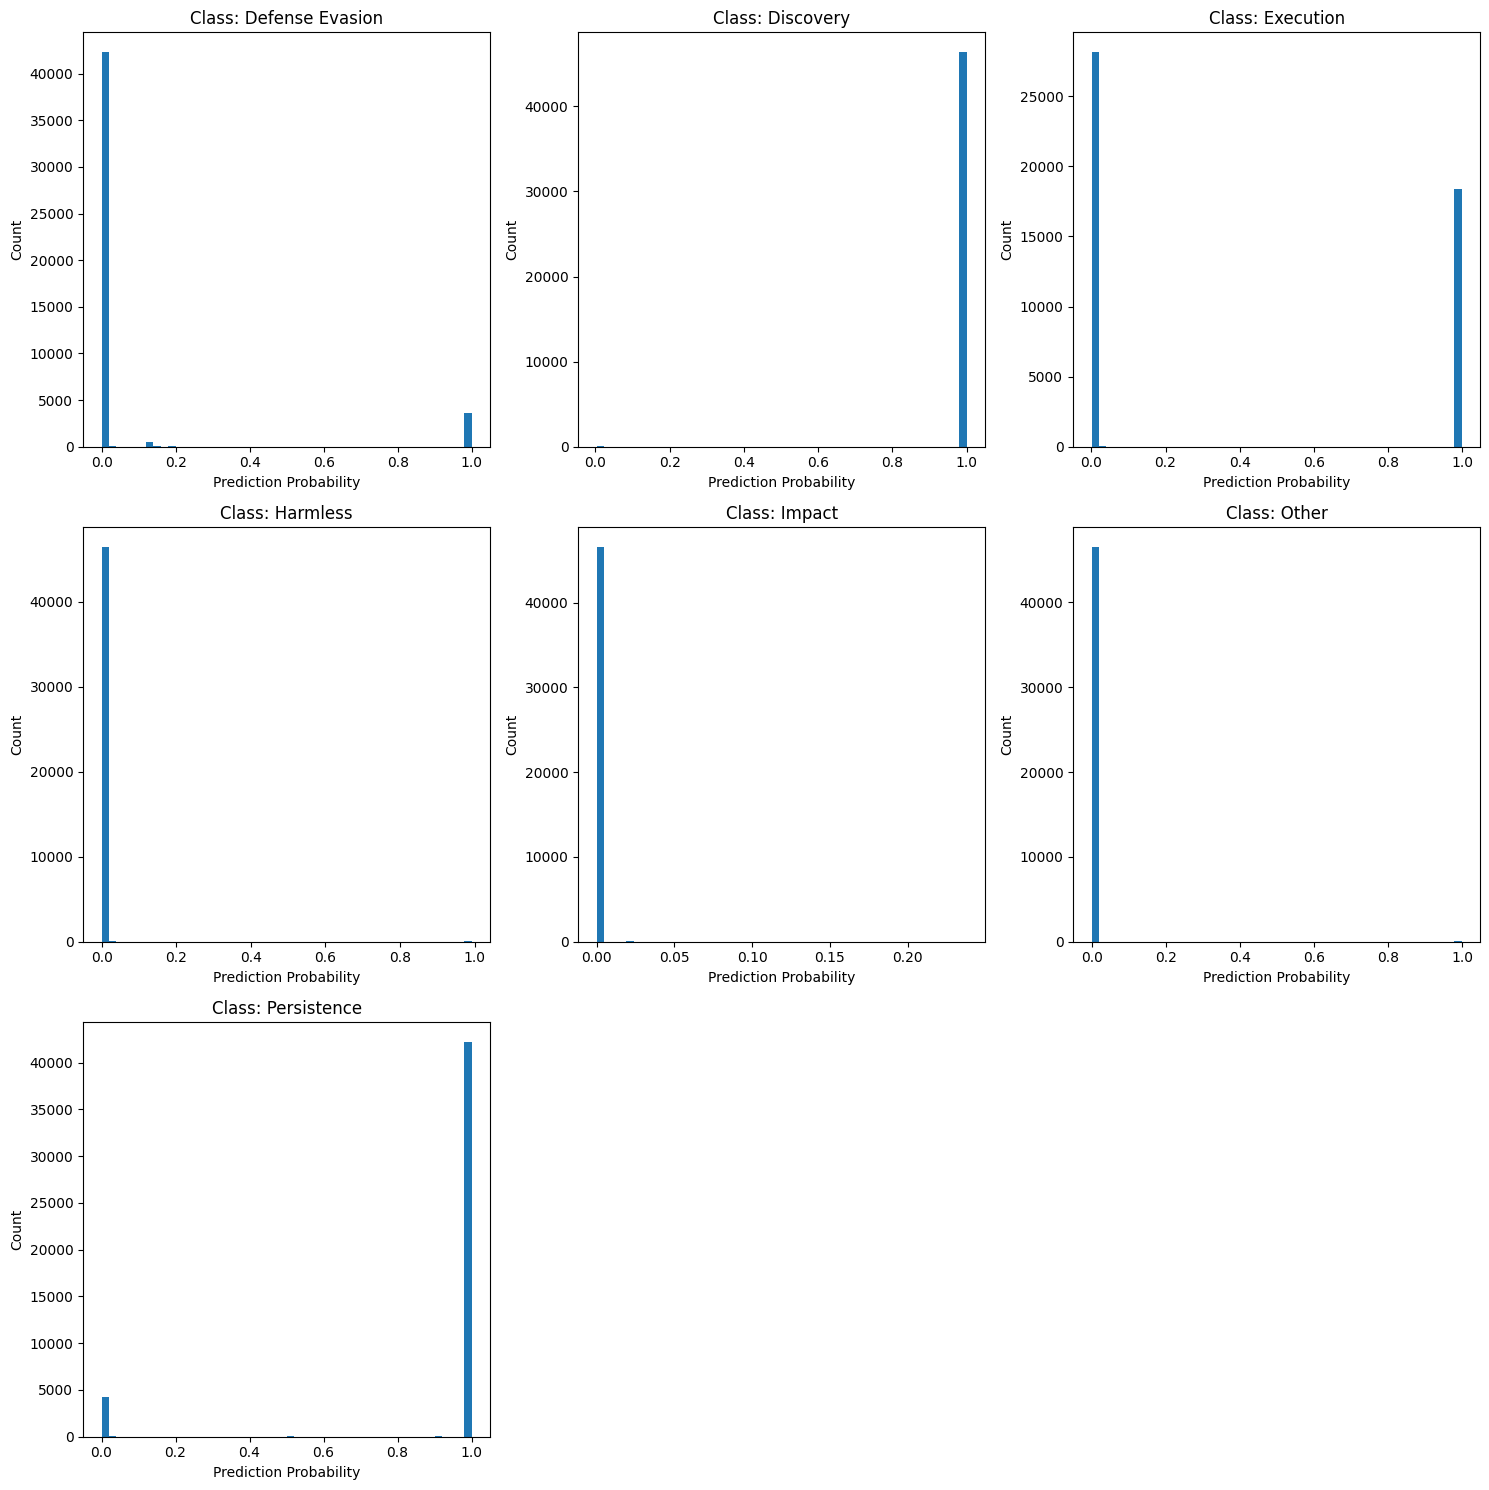
\includegraphics[width=0.7\textwidth]{../figures/plots/section4/probability_histograms.png}
            \caption{Distribution of prediction probabilities for each class showing the model's confidence in its predictions.}
            \label{fig:pred_prob}    
        \end{figure}
        
    \subsection{Recommendations for Model Improvement}

        Based on the analysis, several potential improvements could be considered:

        \subsubsection{Class Imbalance Mitigation}
        
            \begin{itemize}
                \item Implement class weights or sampling techniques for Harmless and Impact classes
                \item Consider data augmentation for underrepresented classes
            \end{itemize}

        \subsubsection{Model Architecture}
        
            \begin{itemize}
                \item Experiment with different BERT variants
                \item Consider ensemble approaches for improving performance on challenging classes
            \end{itemize}

        \subsubsection{Training Strategy}
        
            \begin{itemize}
                \item Implement curriculum learning for difficult classes
                \item Explore different learning rate schedules
                \item Consider longer training with early stopping
            \end{itemize}

        \subsubsection{Data Quality}
        
            \begin{itemize}
                \item Review and potentially relabel samples in the Impact class
                \item Analyze misclassified examples in the Harmless class
            \end{itemize}
    